\chapter{Background on Biological Collections}\label{biodiversity_data}


% Biological Collections Data
% ---------------------------
% Characteristics of occurrence data?
%  Punctual data, often obtained in an opportunistic fashion
%  May include collectors field notes.
%  Main assets of a occurrence record: taxon, location, datetime {Graham2004} -> for us, also collectors
%  Biological collections
%  Data collection is typically opportunistic.
% \cite{Hardisty2013}.

% Biological collections
Biological collections are scientific repositories where biological materials, in the form of physical specimens, are systematically deposited and preserved to be used for scientific purposes. 
Throughout this text we use the term ``biological collections''\footnote{We occasionally also use the term ``museums'', for short.} as a synonym for \textit{Natural History Collections (NHC)}, the later being more widely adopted in biodiversity informatics literature.
Such collections are typically hosted and curated by institutions like herbaria and natural history museums, which provide appropriate physical infrastructure and human resources for ensuring both the long-term preservation of the collections and their accessibility to the scientific community.
%In addition, these institutions usually count with large networks of associated contributors, including professional collectors and taxonomists.

A list with 72 potential uses of herbaria has been compiled by \citeonline{Funk2004}, including for research, education and training, science outreaching.
Biological collections are also a possible data source for studying the history of explorers and expeditions for documenting biodiversity \cite{Funk2004}. 

% Data acquisition: (1) New collecting expeditions; (2) Collections exchanges materials with other institutions



In this chapter we give an overview of how data in biological collections is structured.
We describe the semantics of species occurrence records in section \ref{section:occurrence_data}.
We also discuss some aspects regarding the quality and limitations of such data, and how we deal with these limitations.
Before delving into the characterization of biodiversity data we first review the definitions of some domain-specific terms that will be used throughout this text. 

% =====================
% Terms and Definitions
% ---------------------
\section{Biodiversity-related terms and definitions} \label{section:biodiversity_terms}

Throughout this work we use definitions from the \textit{International Code of Nomenclature for algae, fungi and plants} (ICN) \cite{McNeill2012}. This document outlines a set of rules and guidelines for scientifically naming and grouping plants, fungi and algae, consisting of a universally adopted reference by the botanical scientific community. Nomenclature best-practices for other groups of organisms are governed by other (though similar) documents.

\paragraph*{Taxonomy.}
Within the domain of biology, taxonomy is, in a general sense, the science of classification of organisms. 
Organisms are classified according to their shared characteristics using a hierarchical system, in which organisms are grouped at distinct levels of specificity (or \textit{taxonomic ranks}).
Groups of organisms that are more specific are nested within broader ones. 
For an analogy with set theory, a taxonomic classification system can be thought as being similar to a hereditary (or pure) set, in that all members in a set are, recursively, also required to be sets.

\paragraph*{Taxonomic Rank.}
The taxonomic rank of a grouping of organisms is the level of the taxonomic hierarchy at which it is defined. The most relevant ranks adopted in botany (in descending hierarchical order) are \textit{Kingdom}, \textit{Phylum} (or \textit{Division}), \textit{Class}, \textit{Order}, \textit{Family}, \textit{Genus}, \textit{Species}, as stated in \textit{Art. $3.1$} of ICN.

\paragraph*{Taxonomic Resolution.}
The taxonomic resolution of a biological sample is the taxonomic rank of the most specific taxonomic determination that has been assigned to it.
For instance, if a sample has been determined up to the level of \textit{species}, this rank is also its taxonomic resolution.
As taxa relate to each other on a tree-like hierarchical structure (with each child taxon having exactly one parent, while a parent taxon can have one or more children), taxonomic identities of a specimen at ranks higher than its resolution can be directly determined.
Although this term is not included in the ICN document, we use this definition throughout this text.

\paragraph*{Taxon.}
A taxon is a taxonomic group of organisms at the level of any rank, which are considered by professional taxonomists to form a \textit{taxonomic unit}. Plural is \textbf{taxa}.

\paragraph*{Species.} % ICN Art.23
Species is one of the taxonomic ranks organisms can be determined by professional taxonomists as belonging to. It is regarded to be a basic unit of taxonomic classification, although organisms can be further classified in lower-hierarchy taxonomic ranks (\textit{i.e.}, infraspecific ranks).
Differently from other ranks, the name of a species is composed using a binomial nomenclature system, composed of the name of the genus followed by a \textit{specific epithet}, \textit{e.g.} \textit{Caryocar brasiliense}, \textit{Myrcia guianensis}, \textit{Solanum lycocarpum}.

\paragraph*{Specimen.}
When botanists sample organisms in field they either collect part of the organism (\textit{e.g.} a branch of a tree), the entire organism (\textit{e.g.} the entire body of a weed) or multiple individuals of the same type (\textit{e.g.} a bunch of identical, very small-sized mosses). 
Any of these collected biological materials is an evidence of the existence of a particular organism at some place and time, and should be properly deposited in a biological collection for being preserved as a reference. 
A specimen is defined as one of such evidences, and refers to a punctual observation of a single kind of organism. 
For the formal definition refer to \textit{Art. $8.2$} of ICN. 
Although a specimen could be classified by a taxonomist as being a representative of a given species, this is not a requirement for it to be included in scientific collections. Although taxonomists classify specimens in a best effort manner (the most taxonomically precise as possible), sometimes only higher ranks can be determined. The highest taxonomic rank at which the specimen could be identified is known as its \textbf{taxonomic resolution}.
After properly deposited in a biological collection, each record receives a taxonomic identification that assigns the individual to a \textbf{taxon}.







% ===============
% Occurrence Data
% ---------------
\section{Species occurrence data} \label{section:occurrence_data}
Physical specimens stored in biological collections (also referred to as \textit{vouchers}) are often associated to complementary information, either annotated by the responsible collectors during the collecting act; or annotated at later stages, after the specimen is deposited in the collection \cite{Chapman2005}.
Information from the collection event include the \textit{date, time} and the \textit{geographic location} where the specimen was collected; the names of the \textit{collectors} who were involved in the collection event; and eventual \textit{field notes} describing contextual remarks, such as weather conditions, habitat features, or the sampling method used.
Other crucial piece of information is the \textit{taxonomic identity} of the specimen, determined by taxonomists after the biological material is incorporated to the collection.
%
The taxonomic identity of a specimen includes not only the taxon name assigned to the sample, but also its nomenclatural status and authorship, the name of the taxonomist who has identified the specimen, and other quality-related information.
As the taxonomic identity of a specimen can be re-evaluated by specialists several times after the first determination (though it requires that the investigator has access to the physical specimen), a history of determinations is usually stored in the collection.
%
% Occurrence data
Vouchered specimens, together with their associated data, is what scientifically testifies a punctual observation of a species by a collector, at some location and at some point in time, and is thus referred to as a \textit{species occurrence} record (Figure \ref{fig:occurrences_er}).

\begin{figure}[h!]
  	\centering
    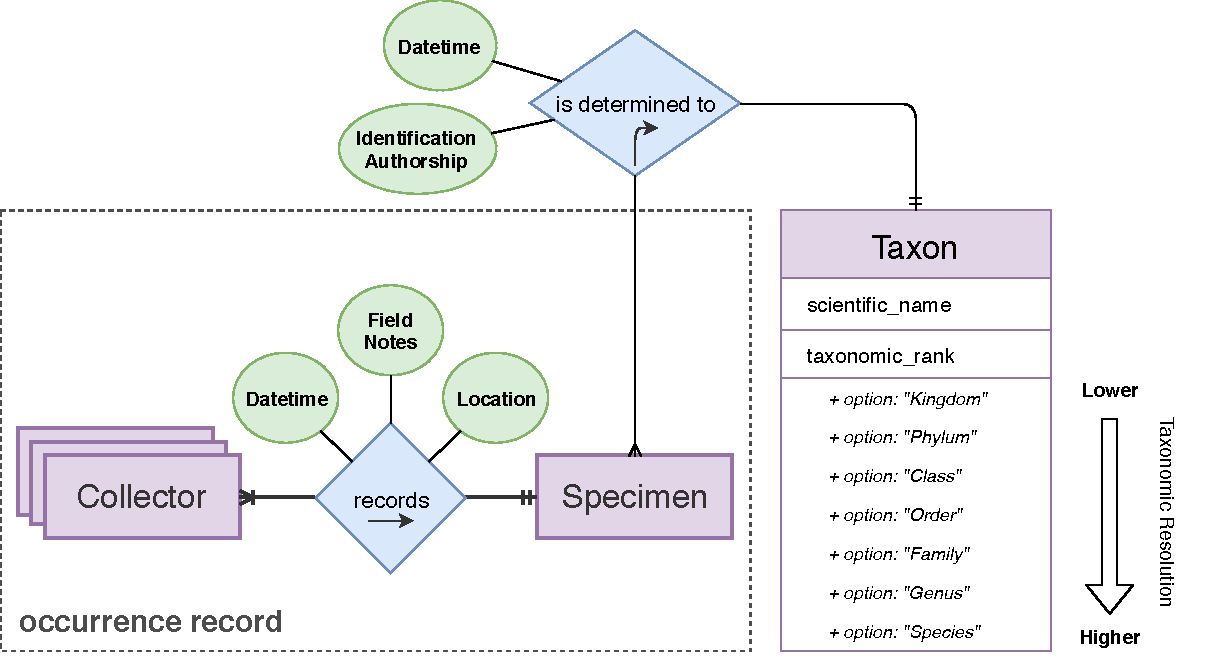
\includegraphics[width=\linewidth]{figures/collections_data/occurrences_er.pdf}
    \caption[Entity-relationship diagram illustrating the main features of occurrence records]{Entity-relationship diagram illustrating the main features of occurrence records. The cardinality of relationships is represented using the Crow's foot notation.}
    \label{fig:occurrences_er}
\end{figure}

% Species occurrence is not exclusive of biological collections Chapman2005b
%% Citizen science and informal collectors
Although biological collections have traditionally been the most traditional sources of species occurrence data, recent advances in mobile computing technology, associated to connectivity of devices to the World Wide Web, have leveraged the participation of informal groups of nature observers in recording biodiversity \cite{Silvertown2009}.
The nature of such records is similar to those from biological collections in that they are punctual observations of specimens in nature, but also have some important distinctions: (i) as nature observers usually do not collect biological materials, there are no vouchered specimens, which difficults the taxonmoic determination of the recorded specimen; (ii) taxonomic determinations result from a collaborative community, not and not by professional taxonomists. 

With the development of electronic databases over the last $40$ years, many institutions have adopted computerized systems for improving the management and accessibility of specimens-related data \cite{Sunderland2013}.
However, in many regions (including Brazil and China) we face challenges on digitizing information, information is not yet digitized or integrated \cite{Meyer2016}.
% Data sharing intiatives




% Data sharing/integration
Data aggregation initiatives have addressed this limitation by facilitating data sharing and integrating many data sources (data aggregators). % data ggregators have already been mentioned
However, integration can only happen when we have data \textit{interoperability}.
Some intitiatives such as TDWG provide biodiversity informatics data standards for data integration and sharing.
DwC is the Darwin Core metadata scheme, and consists of data domains. % check Veiga2014 for refs
% TDWG first mentioned here 

Darwin Core (DwC) is a body of standards, designed to provide a consistent vocabulary for representing biodiversity-related information and making it exchangeable, accessible, reusable and interoperable \cite{Wieczorek2012}.
It has been adopted as an standard for data publishing.
It is an extension of the Dublin Core Metadata Initiative (DCMI\footnote{\url{http://dublincore.org/}}), specifically created for dealing with biodiversity data.
composed of many terms to designate \textit{classes} and their \textit{properties}.
Terms are divided into record-level terms, which ; and auxiliary terms.
The \textit{Occurrence} class is used
An occurrence event is represented in DwC with the \textit{Occurrence} class.






\section{Limitations of data} % Newbold2010 James2018 Hortal2007
% Presence vc presence-absence data
% Collectors Behavior (TerSteege2011)
% Limitations: sampling bias, lack of assessment of sampling effort, lack of geographic coverage
% Name ambiguity issue Groom2014

% Most species remain poorly collected , Nelson1990 TerSteege2011

% ===========
% Data issues
% -----------
Biological collections are still the main sources of biodiversity data.
Despite the many caveats associated to museum data, they cannot be ignored, as they are still the main sources of information about the distribution of species, and thus are relevant for a multitude of ecological and conservationist investigations, including for the selection of high-priority biodiversity regions \cite{Funk2002}... 
Although biodiversity scientists have undoubtedly benefited from open access to massive volumes of species occurrence data from many biological collections, there are some caveats that must be accounted for, before using data for modeling.
Efforts are necessary for making them usable, as biodiversity data is hard to gather \cite{}.
Data must be cleaned before used.
% Data quality
Dealing with so many heterogeneous data sources also introduce new complexities related to data.
Data is not always adequate for investigating every aspect of natural systems.
Using inadequate data for studying specific aspects of biological diversity can lead to erroneous or misleading results \cite{Chapman2005}, and investigators must be aware of the inherent limitations of their data before formulating their questions. % Chapman in pg. 1

% charact. 1: Wallacean Shortfall (coverage of data)
Availability of detailed information is still very scarce for most known organisms.
This scenario, referred to as the \textit{Wallacean Shortfall} \cite{Lomolino2004}, is even more critical for megadiverse countries, which still remain largely unexplored for many regions and taxonomic groups \cite{Soberon2004}.
The lack of sufficient data for threatened species is even more concerning, as designing efficient programs for their conservation require knowledge on their geographic distribution and ecological requirements.
This shortage of data, combined with the non-systematic sampling and insufficient quality limits the use of data from biological collections for many intended applications, many of which require an intensive amount of data to be available \cite{Guisan2007}.
% Guisan2007 -> Many applications require high volumes of data, low sample size reduces the performance of many techniques
% Galante2017 -> Techniques for SDM using few records
In the context of the present work, sampling biases and the quality of data are central.


\subsection{Sampling biases}
% charact. 2: Non-uniform sampling effort -> Lead to bias
One important aspect that often limits the usability of primary data from biological collections concerns the way in which it is gathered in field.
In general, most species occurrence data composing biological collections derive from exploratory field expeditions, in which organisms are recorded in a non-systematic \textit{observational} fashion by different collectors, using different methods and at distinct circumstances (though records resulting from experimental studies are eventually incorporated in museums as well). 
As a result, the distribution of sampling effort in such datasets is uneven and rarely quantified, leading to \textit{sampling biases}.

As defined by \citeonline{Chrisman1991}, biases are uniform shifts in measured values, resulting from systematic errors that are introduced by some measurement system.
They are expressed as unrealistic tendencies in data, and can usually be mitigated with the adoption of random sampling designs.
%
Sampling bias in biodiversity data can be classified into several distinct categories, depending on the aspect of data under investigation \cite{Daru2017}.
Here we briefly present four of them, the first two (collector and taxonomic biases) being the most relevant in the scope of our work.
%
% collector bias, taxonomic bias, (geographic bias, trait bias, historical bias, seasonal bias) % Daru2017, Haripersaud2009 
\paragraph*{Collector bias.}
Not all collectors contribute to the same extent to biological collections.
In fact, it has been observed that a considerable percentage of records in biological collections are gathered by only a small subset of very productive collectors, while the vast majority of collectors contribute with just a few records, each \cite{Daru2017,Carine2012}.
This unbalance in the representativity of collectors is what defines the \textit{collector bias} in biological collections.
As the overall taxonomic composition of collections --- as well as the geographical and temporal distribution of their records --- tend to reflect the particular interests and collecting behavior of their most representative collectors, collector bias propagates to other categories of biases in the collection. Therefore, we consider that characterizing collector bias is a fundamental step towards understanding other types of biases.

\paragraph*{Taxonomic bias.}
Not all taxa are quantitatively represented in biological collections in the same proportions as they occur in natural systems.
Instead, the taxonomic composition of collections reflect the interests and collecting behavior of the communities of collectors contributing to them.
Taxonomic bias is intrinsically related to collector bias, as the overall composition of biological collections tend to reflect the interests of their most productive collectors.
The collection is biased towards taxonomic groups most sampled by the most productive collectors.
%
Rare species tend to be more overrepresented in biological collections in comparison to common species \cite{}.
%
%Some studies have proposed to assess taxonomic bias of collectors by comparing the representativity of each taxon on their sets of records to the herbarium \cite{Haripersaud2009}. %Such approaches give at most a view of how well a collector represents the composition of the collection.
%However, if we consider the herbarium itself is composed of contributions of multiple collectors each with particular interests --- and therefore also biased ---, the herbarium is biased, not representing well the natural communities.
%As it is very common that collectors towards sampling the highest number of species as possible in localities they visit, the collection is non-random, and rare species tend to be overcollected and common species, undercollected \cite{TerSteege2011}.
%Biases of the most productive collectors would be hard to assess.

\paragraph*{Geographic bias.}
% [Kadmon, R., O. Farber, and A. Danin. 2004. Effect of roadside bias on the accuracy of predictive maps produced by bioclimatic models] 
Collection sites are not randomly selected in geographic space, nor they are all sampled to the same extent.
As features of the landscape make some areas more accessible for collection activities than others \cite{Hijmans2000}, collectors tend to prioritize those to maximize their productivity while minimizing costs.
Geographic bias arises as a consequence of non-uniform collecting effort in geographic space, and tends to reflect the preferred locations of the most productive collectors.
Some regions that are more accessible being thoroughly sampled (such as areas near urban centers, roadsides and margins of rivers);
while others which are more inaccessible, such as rainforests, being only poorly or not sampled at all.
%
Geographic bias is also observed at broader scales.
A compilation of the representativity of plants in GBIF by \citeonline{Meyer2016} has shown that among the most representative countries and regions are the United States (mainly the west coast), Central America, countries in Europe (including the nordic countries), Australia, Japan, New Zealand.


\paragraph*{Temporal bias.}
The recording activities of collectors are not uniformly distributed over time.
The patterns of activities of collectors change in time, in function of their personal characteristics (\textit{e.g.} age, stage in career)
Collectors show preferences and and face difficulties on performing 
Temporal bias can be further subdivided into two more specific classifications (although there are others):
Historical bias. 
Seasonal bias: Two causes: 
Biases in higher granularities, such as weekdays/weekends...
Collectors also tend to concentrate their activities around the best seasons for fieldwork.



Building models without accounting for biases in data has been observed to strongly impact their performance, leading to spurious results which can be misinterpreted and, ultimately, lead to wrong decisions.
For instance, assessing patterns of species richness from species occurrence datasets has been shown to be particularly challenging due to geographical bias in data \cite{Hortal2007,Reddy2003}, as higher diversities tend to be observed at more accessible sites due to higher sampling effort.





% Two shortcomings: presence-only data and representativity
% Presence-only data and richness

Non-uniform sampling effort also makes it hard to infer true absences from biological collection datasets.
As the distribution of sampling effort towards locations is not known in biological collections, its data is regarded as `presence-only', which means that the absence of a record for a species at some location does not necessarily indicate that the species is truly absent \cite{Graham2004}.
Instead, no collectors that would potentially be interested on recording it have visited the location.

% Representativity
Another problem arising from non-uniform sampling effort concerns the representativity of species in biological collections.
Collectors seldom collect more than one exemplary of each species at the same place in the same expedition, and thus species representativity in museums do not correspond to their abundance in natural systems \cite{TerSteege2011}.
Thus, common species are not always more representative than rare species.
In fact, rare species are eventually more represented than common ones due to the fact that more experienced collectors tend to prioritize collecting rare over common ones \cite{Nelson1990}.
% Problems in modeling
Using presence-only data for assessing richness is problematic, although there are methods for overcoming this limitation, as most records available for specimens are presence-only \cite{Zaniewski2002}.
Richness was observed to be correlated to survey effort, richness is biased towards regions that are more thoroughly sampled \cite{Hortal2007}.







% charact. 3: Data quality
% Briefly describe the limitations due to errors








\subsection{Data quality}
Besides the limitation on the availability of data, another limitation concerns its \textit{quality}.
A definition for data quality which considers its \textit{fitness for the intended use} was first proposed in the context of geographical information systems \cite{Chrisman1984} and became widely adopted by the BI community.
In BI, data quality is defined as its fitness for the intended use, and thus assessing quality depends on first defining the intended use of data (data fit for use).
A dataset is fit for use if it is suitable (or valuable) for answering a given question.
Data is considered to be high quality if the desired information can be obtained from it.
Thus, quality is not an exclusive attribute of the dataset, but also depends on the requirements of users.
%
A framework for systematically describing the ``fitness for use'' from the perspective of the user is proposed by \cite{KochVeiga2017}. 
The framework is based on a ``Fitness for Use Backbone'' (FFUB)
%
%
Data quality loss can be affected in multiple stages of its life cycle \cite{Chapman2005}, including the moment of the recording event, its preparation before it is incorporated, the taxonomic determination, data documentation, data digitization, data storage and analysis.
%
Before being used, data quality must be assessed, which depends on the user needs.
Users need a systematic way to both assess and manage data quality.
\citeonline{KochVeiga2017} have proposed a framework for systematically assessing requirements that make quality acceptable for each kind intended use, in the biodiversity informatics community.


Increase the usability of a dataset, making it suitable for answering a wider range of questions.
% Veiga2014 -> Identified and defined the main dimensions of data quality and their associated problems 
Although data quality can be improved by either prevention or correction, being the prevention considered more effective, as correcting the data is costly\cite{Chapman2005}, prevention is out of our scope, here we limit our scope to correction.
Here we deal with data validation and cleaning of aspects that are most relevant for the modeling we propose.
GBIF has a set of data validation routines, that base on outlier detection, that look for inconsistencies and flag them, but do not overwrite, so that they can be inspected by data user.

% Errors
Errors in biological collections datasets can be of distinct types, and are more common on the taxonomic identity and spatial information, and can be manually inspected by comparing with collector field notes \cite{Graham2004}.
Some of the most common problems include the wrong identification of specimens; using outdated taxonomy; bad georreferencing of records \cite{Soberon2004}.

% Data problems
\citeonline{Dalcin2005,Veiga2014} have assessed the most common data quality issues in species occurrences datasets, and identified eight recurrent patterns of problems.%, observable across multiple data domains. 
We review five of them which are most relevant for our purpose:
(\textit{i})~\textbf{domain value redundancy}, when multiple distinct values in the dataset redundantly represent the same real-world entity;
(\textit{ii})~\textbf{non-atomic data values}, in case a value semantically contains multiple instances of the fundamental piece of information it should represent (an atomic value is regarded as being indivisible);
(\textit{iii})~\textbf{inconsistent data values}, in case they do not follow a strict standard, eventually leading to contradictory information;
(\textit{iv})~\textbf{incorrect data values}, when erroneous information are inserted in the dataset; and
(\textit{v})~\textbf{missing data value}, in case values at some field are absent (\textit{i.e.} null values).

% Data completeness: Funk1999 Jacobs2017 Soberon2007
% Data quality dimensions

They have also proposed mechanisms for preventing the inclusion of errors and uncertainities during the data entry, as a measure for the improvement of data quality.




%
\paragraph*{Taxonomic errors.}
The accuracy of taxonomic determinations depend on the expertise of the taxonomists who evaluate the specimens.
Determination issue, as many specimens are incorrectly identified;
The accuracy of the taxonomic determination depends on the expertise of the taxonomist.
if the identification of the specimen is incorrect, and can be reevaluated if the physical specimen is available.
Typographic (misspelling) errors are particularly common.
They can be dealt with during data entry, by using authority files containing accepted names 

\paragraph*{geographic errors}commonly associated to 
wrong coordinates, 
imprecise coordinates(e.g. if the coordinate was not originally recorded, and is later inferred as the centroid of a municipality or state), 
unknown datum, 
null values being interpreted as (0,0) coordinates.
%
\paragraph*{temporal errors.}
%
There are also \textit{typographic} errors, which are common for example in the taxonomic names and in other fields, such as the collector field.

\paragraph*{inconsistencies in fields.}




\section{Data requirements for network modeling} % What should I do for improving data quality for SCN and CWN modeling
In this section we describe some potential issues and requirements that must be observed in species occurrence datasets (Figure~\ref{fig:occurrences_er}) for the purpose of modeling Species-Collector Networks (SCNs) and Collector CoWorking Networks (CWNs).
We base our description on the \textit{data quality needs} as recommended by \citeonline{KochVeiga2017} for modeling SCNs and CWNs.
Our models are constructed basically require two \textbf{information elements}: the names of collectors and the taxonomic identity of the specimen at each occurrence record.
In a dataset following the DwC standards body, collector names and taxonomic identities should be found under the terms \textit{recordedBy} (class \textit{Occurrence}) and \textit{scientificName} (class \textit{Taxon}), respectively.
%
In SCNs, each record containing a set of collectors and a taxon. 
Interest ties are extracted from each record, linking each collector to the taxon.
More details in section \ref{subsec:scn-model-construction}.
%
In CWNs, only the collector field is required.
For each record, collaboration ties are created (or reinforced) by combining all collectors in a pairwise fashion.
More details of the construction process are provided in section \ref{section:cwn_construction_fromdata}.
%
Here we discuss data requirements for modeling our network models, and how to manage data quality for that purpose.

As the collectors field is not very often used for BI applications, its quality is seldom assessed, neglected by data curators.



% The collector field
\subsection{Collectors' names}\label{section:data_req_collector}
This information element contains the names of all collectors who were responsible for a species occurrence record.
From the field data domain \cite{Dalcin2005}.
In a DwC-compliant dataset, collectors names should be found under the term (or field) \textit{dwc:recordedBy} (within class \textit{dwc:Occurrence}), formatted as a list of collectors names concatenated into a string, using the vertical bar (` | ') as the delimiter.
For instance, a record authored by `M.A. Silva' and `N.T. Souza' would contain a string with value ``M.A. Silva | N.T. Souza''.
However, storing multiple names into a single string makes values in this field \textit{non-atomic}, thus requiring additional processing for the retrieval of individual names.

% names atomization
We refer to the process of extracting multiple names by splitting the string on a delimiter character as the \textbf{names atomization} routine, which is mandatory for our use case.
Applying the names atomization process to an entire dataset should be a trivial task if a consistent and non-conflicting delimiter (though not necessarily the vertical bar) is adopted throughout the entire dataset.
However, we suspect this is rarely the case for most species occurrence datasets.
Atomization issues arise when the atomization routine is unable to systematically distinguish names in a string, leading to the representation of unrealistic entities in the model.

% naming conventions
Using inconsistent (or ignoring) \textbf{naming conventions} while registering collectors names in a dataset is also potentially problematic, as it makes it more difficult to systematically interpret names and extract their component parts.
Naming conventions are rules used for shortening (or simplifying) names before they are inserted in the database.
One common practice is to abbreviate the first and middle names of collectors, while keeping the last name unabbreviated.
Under this convention, for instance, the name `João Souza Silva' would be mapped to `J.S. Silva'.
As collectors are not always aware of the naming convention adopted at the collection, they often include collectors names in their field notes using their own convention or, in the worse case, not using conventions at all.
The task to assure that all records are properly formated is therefore assigned to system managers, who must inspect and fix each entry manually before including them in the dataset.
As a result, names are eventually registered with typographical errors or being inconsistent with the adopted convention, although some database management systems are able to assist users in this aspect by parsing input names or by suggesting similar names that have already been registered.

% Heteronymous: result of unconsistent naming convention
Another negative effect of inconsistently formating collector names is the insertion of multiple \textbf{name variants} to the same real-world entity.
This can also be the result of typos (e.g. souza becoming souza), or simply omiting parts of the name (e.g. if there are two collectors, A.M.Souza and A.P.Souza, omitting the middle initial makes their names indistinguishable).
%
The \textbf{entity-resolution} problem concerns the mapping of name variants that refer to the same real-world entity.
\citeonline{Groom2014} came across the same problematic, considerable variations in the formats of names.
They used a names cleaning routine in which they merged all variants of names which could be unambiguously mapped to a single person, while excluding those which could not.
This problem was also tackled by \citeonline{EstevaoDaSilva2016} by using a data mining methodology, based on association rules analysis, for identifying possible name variants.
The method consists of observing 

% Homonymous
Assuming that all records in a dataset are consistent with some naming convention and that they use the same character for delimiting names (\textit{i.e.}, names can be properly atomized), distinct real-world entities may still end up being registered under the same name.
These entities, which we refer to as being \textbf{homonymous}, are also problematic for our use case, as they are incorrectly represented in the network models as a single entity.
In case the naming convention requires the abbreviation of parts of the names, homonymous can be created in the database from two names that are originally distinct.
For instance, `João Souza Silva' and `Jorge Soares Silva' would be mapped to a homonymous `J.S. Silva', if both the first and middle names were abbreviated.
%
Some collections include mechanisms in their naming conventions for disambiguating homonymous.
For instance, a complementary field containing unique identifiers for collectors can be appended to each record in the dataset, allowing the identification and resolution of homonymous entities.
Another approach would be making a
assigned to each for collectors can be included in the associated to each collector in the database management system, such that 


% Omission
Finally, some collectors only include their own names in records in which they are first collectors, omitting the names of secondary collectors or, eventually, aggregating them under the expression `et al.'.
We refer to this issue as \textbf{names omission} (within the \textit{completeness} DQ dimension), which strongly impacts as it fails to represent collaborative ties and collecting activities of the collectors who are not listed.


\subsection{Taxon name}
This information element contains the taxonomic identity assigned to the specimen from an occurrence record, being included into the taxonomic data domain \cite{Dalcin2005}.
In a DwC-compliant dataset, the taxon identity should be  DwC, the taxonomic identities assigned to specimens are assigned to the term \textit{dwc:scientificName}, which is part of the \textit{dwc:Taxon} class.
Other relevant elements are \textit{dwc:taxonRank}






% Taxonomic names
In a dataset following DwC, the taxonomic identities assigned to specimens are assigned to the term \textit{scientificName}, which is part of the \textit{Taxon} class.
Other terms under \textit{Taxon} class are eventually also relevant, such as \textit{taxonRank},



In the scope of this work, we primarily deal with the entity-resolution problem.




% Data Aggregators
Gbif provides a data preprocessing routine % https://www.gbif.org/infrastructure/processing





%% As it is common practice for botanists to record each species once during field work, some important ecological attributes such as the species abundance are not to be directly inferred from such data. {check van Gemerden 2005, from Haripersaud2009}


% Biological collections are composed of aggregates of multiple biodiversity surveys, each recorded with particular methodologies
% Records sampled using distinct methodologies can be combined for optimizing data use \cite{VanGemerden2005}.











% ============
% Data quality
% ------------
% [Soberon2004]

% Data quality among collection records is uneven -> worse for large datasets and for datasets composed by multiple sources
% Procedures are needed for correcting problems

% Quality issues: 
%% Determination issues: many specimens are incorrectly identified;
%% outdated taxonomy;
%% georreferencing errors.

% Data atomicity issues:
% Some fields are not atomic: more than one entity is represented as a single data element. 
% In the recordedBy field, Darwin Core standards state that distinct names should be separated by | (delimiter).
% This varies depending on the standard a collection uses. For example, the BRAHMS system recommends using a ';' as the delimiter.
% BRAHMS docs: https://herbaria.plants.ox.ac.uk/bol/brahms/support/documentation

% Identity issues:
% Entities are not guaranteed to have the same ids through distinct datasets.
% Even in the same datasets there may be variations in their names
% this is specially problematic for fields like the collectors field, which is overlooked for most applications of such data. 
% Some standards provide guidelines for including collectors names: last name + first initials...
% However different standards give distinct guidelines and thus name variants are common.
% How to map all name variants to the same entity? -> This leads to the Entity-resolution problem


% Data fit for use


% =============
% Data cleaning
% -------------
%[Chapman2005a]

% Why do we need data cleaning? -> We must make data fit for its indended use

% Goal: improving data quality, removing or treating entries that are 

% Adopting standardized collectors names
% Checking collectors itineraries -> look for the spatial pattern of records by the collector


% ================
% References
% ----------------
%% Museum-based informatics{Graham2004}



